\section*{Problem 4: Policy Function Approximation in the Neoclassical Growth Model}
\begin{enumerate}
\item
The Lagrangian for households is
\begin{equation}
	\mathcal L=\sum^\infty_{t=0}\beta^t\ln C_t-\lambda_t[C_t+K_{t+1}-(1+r_t-\delta)K_t+w_t]
\end{equation}
The household's FOCs are
\begin{align}
\tag{$C_t$}
	\beta^tC_t^{-1}-\lambda_t\overset{!}{=}0&\implies\lambda_t=\beta^2C_t^{-1}\\
\tag{$K_{t+1}$}
	-\lambda_t+(1+r_{t+1}-\delta)\lambda_{t+1}\overset{!}{=}0&\implies \lambda_t=(1+r_{t+1}-\delta)\lambda_{t+1}
\end{align}
Thus we have
\begin{equation}
	C_{t+1}=\beta(1+r_{t+1}-\delta)C_t.
\end{equation}
For firms, the FOC is
\begin{equation}
	\alpha K^{\alpha-1}_t-r_t\overset{!}{=}0\implies r_t=\alpha K_t^{\alpha-1}.
\end{equation}

\item At equilibrium, both firm's and household's problems are solved. Moreover, at steady state $C_t=C_{t+1}=C$ and $K_t=K_{t+1}=K$. Thus, we have
\begin{align}
	1=\beta(1+\alpha K^{\alpha-1}-\delta)\implies
	K^*=\left(\frac{\beta^{-1}+\delta-1}{\alpha}\right)^{\alpha-1}\approx7.2112.
\end{align}
Due to the market clearing, consumption equals production and
\begin{equation}
	\widetilde C(K)=K^{\alpha}.
\end{equation}

\item See code file \texttt{Q4.m}.

\item See code file \texttt{Q4.m}.

\item See Figure \ref{Q4_5}.
\begin{figure}[htbp]
\begin{center}
	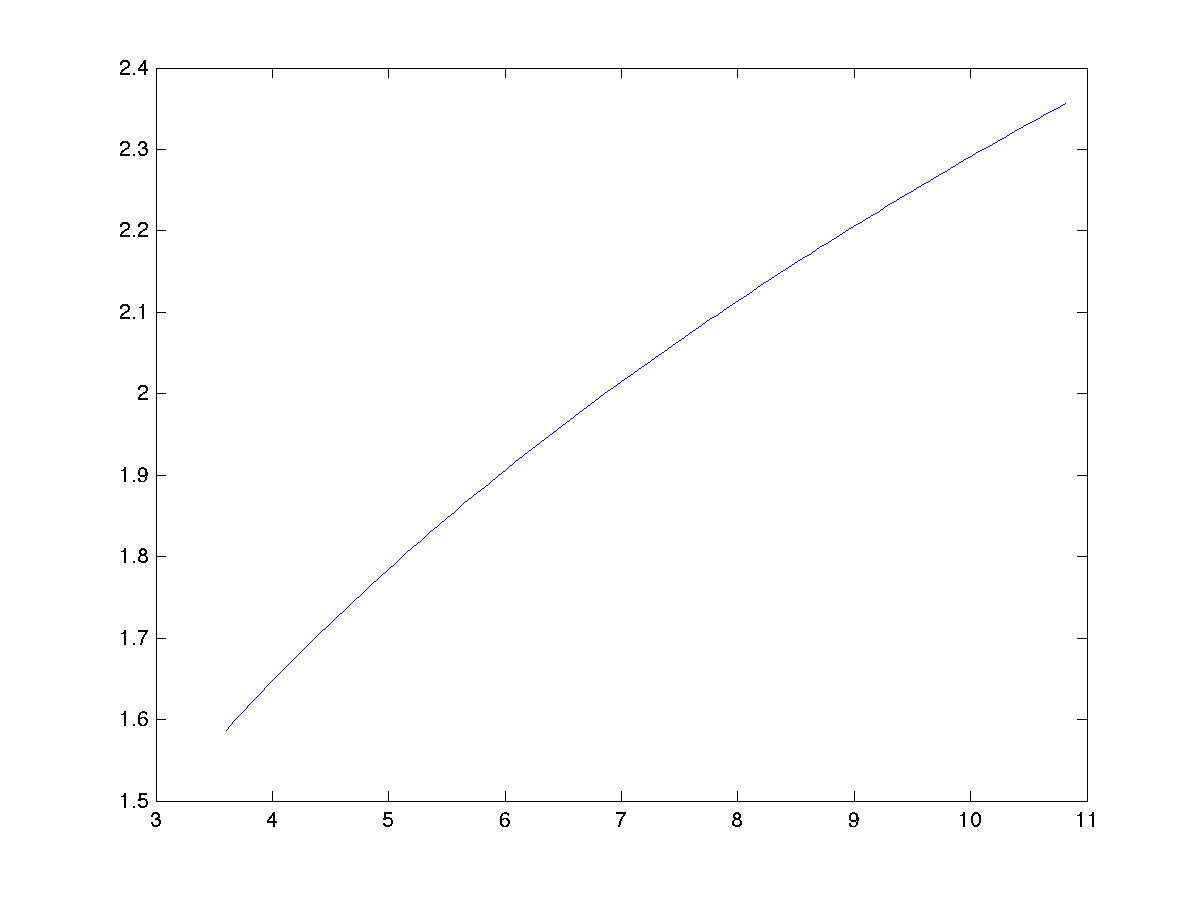
\includegraphics[width=10cm]{Figure/Q4_5.png}	
\caption{Consumption Policy}
\label{Q4_5}
\end{center}
\end{figure}

\item
Capital grows monotonically with decreasing speed towards the steady state. See Figure \ref{Q4_6}.
\begin{figure}[htbp]
\begin{center}
	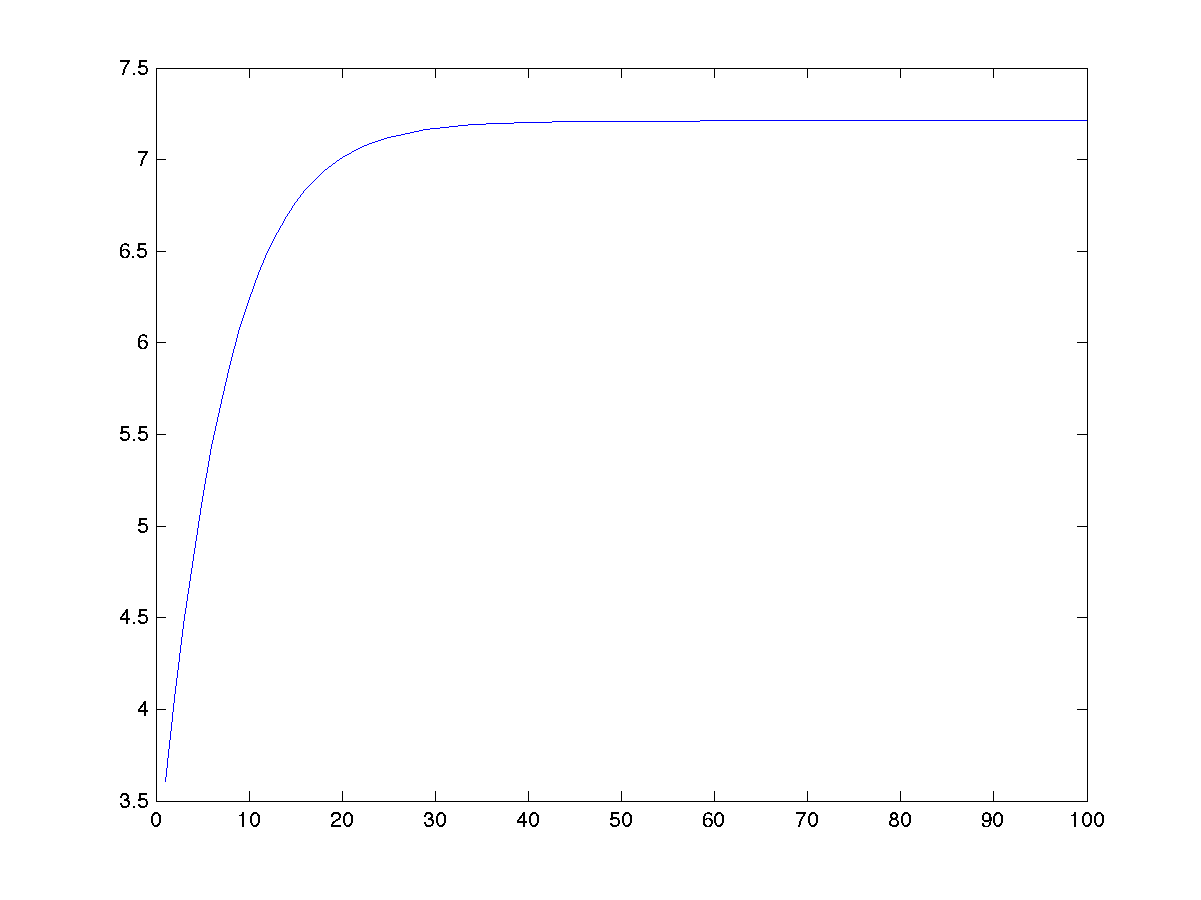
\includegraphics[width=10cm]{Figure/Q4_6.png}	
\caption{Capital}
\label{Q4_6}
\end{center}
\end{figure}

\item
Maximum absolute error = 3.8648e-07.\\
Average absolute error = 7.315e-08.
\end{enumerate}